% PREAMBLE
\documentclass[12pt, letterpaper]{article}
\usepackage[utf8]{inputenc}
\usepackage{tipa}
\usepackage[margin=1in]{geometry}
\usepackage[parfill]{parskip}
\usepackage{hyperref}
\usepackage{graphicx}
\title{Pronunciation Checking with ASR\\ \small User Documentation}
\author{Evan Nichols}
\date{MFF 2021/2022}

\begin{document}
\maketitle

\section*{What Is It?}
This application allows the user to test their pronunciation of various English sentence prompts. It supports multiple concurrent users. Users record themselves, via the web page, and then wait for their pronunciation to be evaluated. The user's speech input is evaluated on the basis of phonemes, which are the smallest units of sound that can distinguish one word from another. After a short delay, they may pull up their score and review, or try again. It uses a neural network module built for automatic speech recognition to evaluate the speech. The module compares the users' spoken phonemes to those of the (converted) text prompt, and reports the differences. The application is built using Flask, a web framework for Python, with a web page run in JavaScript.

\begin{figure}[h!]
    \centering
    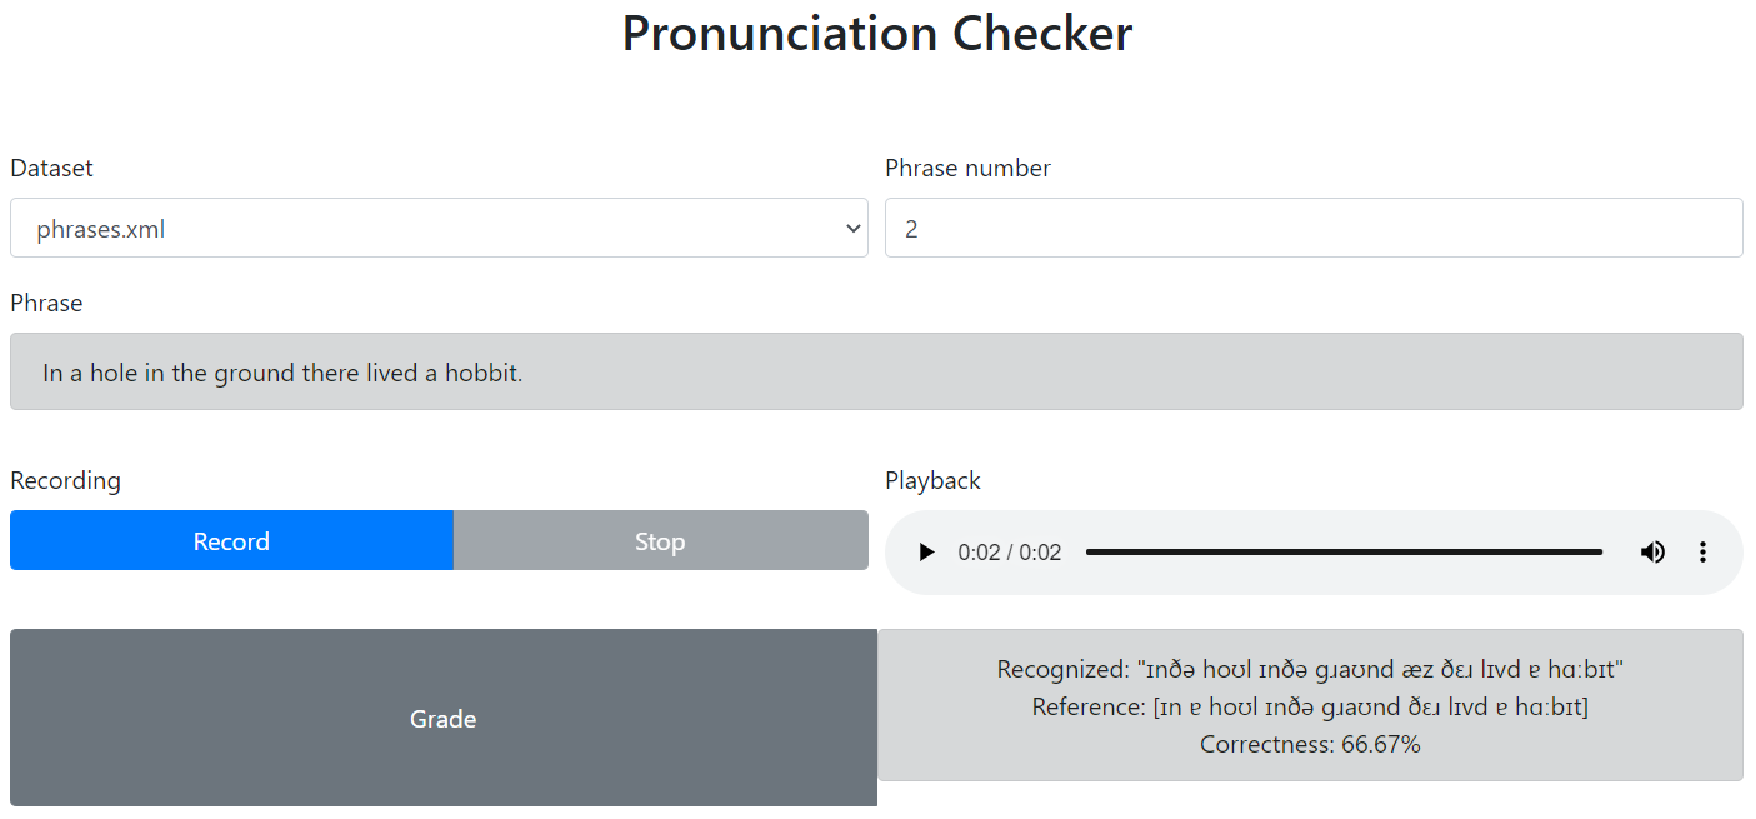
\includegraphics[width=1\textwidth]{images/results.pdf}
    \caption{Web page after user has input speech and received a score.}
\end{figure}


\newpage%######################################################################
\section*{How to Use this Appplication}
Upon loading the web page, the user is presented with a simple interface of a few fields, and will be prompted by most browsers for microphone access. Immediately, the \textbf{Record} button may be pressed. This will begin recording, and the user should read the \textbf{Phrase} text out loud. After speaking the phrase and pressing \textbf{Stop}, the recorded audio is sent to the server-side along with the text prompt and processed and packaged into a data set. This data set is then processed by an automatic speech recognition module and the user's speech audio is graded against the prompt phrase. A score, marking how well the user pronounced the prompt, is stored in a text file and once when the user presses \textbf{Grade} this score is output to them. To add varying challenge, the user may choose from a number of phrases. 

\subsection*{Phrase Prompts}
The phrases can be any English words and sentences. The prompts do not NEED to be legitimate English, but for the sake of pronouncing words well it makes more sense for them to be actual language. Special characters are irrelevant in the grading, as the program strips items such as '!' and ':' before passing the prompt key to the ASR module. The phrases included in the app as of this writing are taken from various books and poems. 

\subsection*{Input Audio}
The user's speech speech is recorded, the raw data is sent to the back-end and then reformatted to a \textit{.wav} file with a sampling rate of 16000 and 1 audio channel. A \textbf{spectrogram} is also created which displays some information to the user. The spectrogram measures frequency (y-axis) over time (x-axis), and the intensity of the color marks the amplitude of the frequency at that moment.

\begin{figure}[h!]
    \centering
    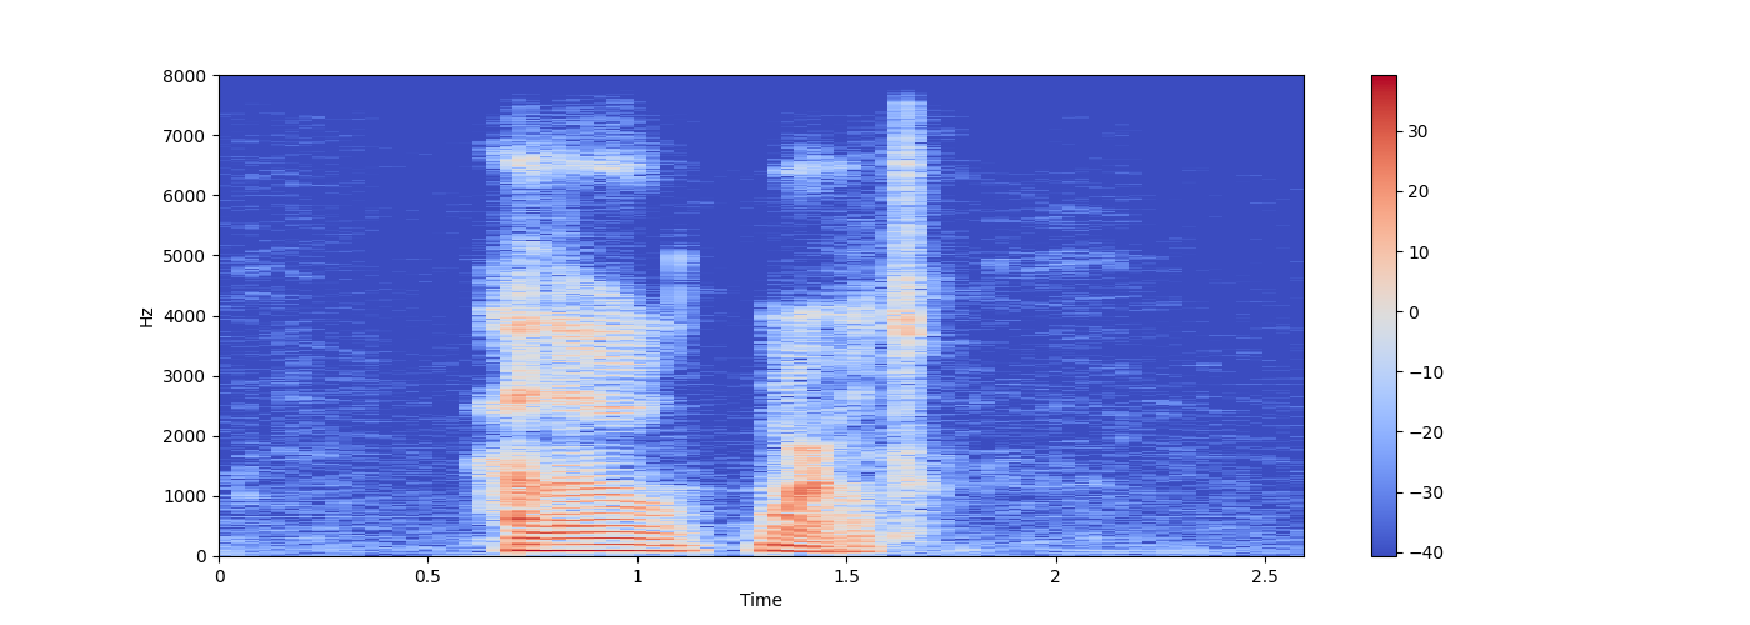
\includegraphics[width=1.1\textwidth]{images/spectro.pdf}
    \caption{Spectrogram for speech "hello world".}
\end{figure}


\newpage%######################################################################
\section*{User Interface}
\begin{itemize}
    \item \textbf{Dataset} is a drop-down list of the available phrase libraries. Each phrase is an item in an XML file with a single id, which denotes the items position in the file (1, 2 etc).
    \item \textbf{Phrase number} is a simple selector, pressing up or down pulls the corresponding phrase from the currently selected library. The selector loops around the dataset.
    \item \textbf{Phrase} is a text box that displays the currently selected phrase. It is this text the user is expected to read out loud. The phrase is sent along with the audio to the ASR module, but before that it is converted to its phonetic representation (phonemes) and stripped of any non-alphabetic characters, eg. '-', or '!'.
    \item \textbf{Record} is a button that begins recording, assuming the user has given microphone access to the browser when prompted. The user should read the text in \textbf{Phrase} out loud, and hit \textbf{Stop} when they are finished speaking. Hitting \textbf{Record} again (after \textbf{Stop}) will overwrite any previous input, allowing the user to adjust their submission.
    \item \textbf{Stop} closes the recording and, behind the scenes, sends the audio and prompt to the back-end and activates the \textbf{Grade} and \textbf{Playback} elements (deactivated by default).
    \item \textbf{Playback} allows the user to review their recorded speech. 
    \item \textbf{Grade} pulls the results from '\{UUID\}\_graded.txt', and displays them to the right. The results include the recognized phonemes (what the user submitted), the correct phonemes (from the prompt), and a percentage score marking grading the user's pronunciation. Since the ASR module requires a variable amount of time to run, based on the size of the input data, a delay might occur between the user pressing \textbf{Stop} and \textbf{Grade} returning the appropriate results, in which case a message communicates this. 
\end{itemize}

\begin{figure}[h!]
    \centering
    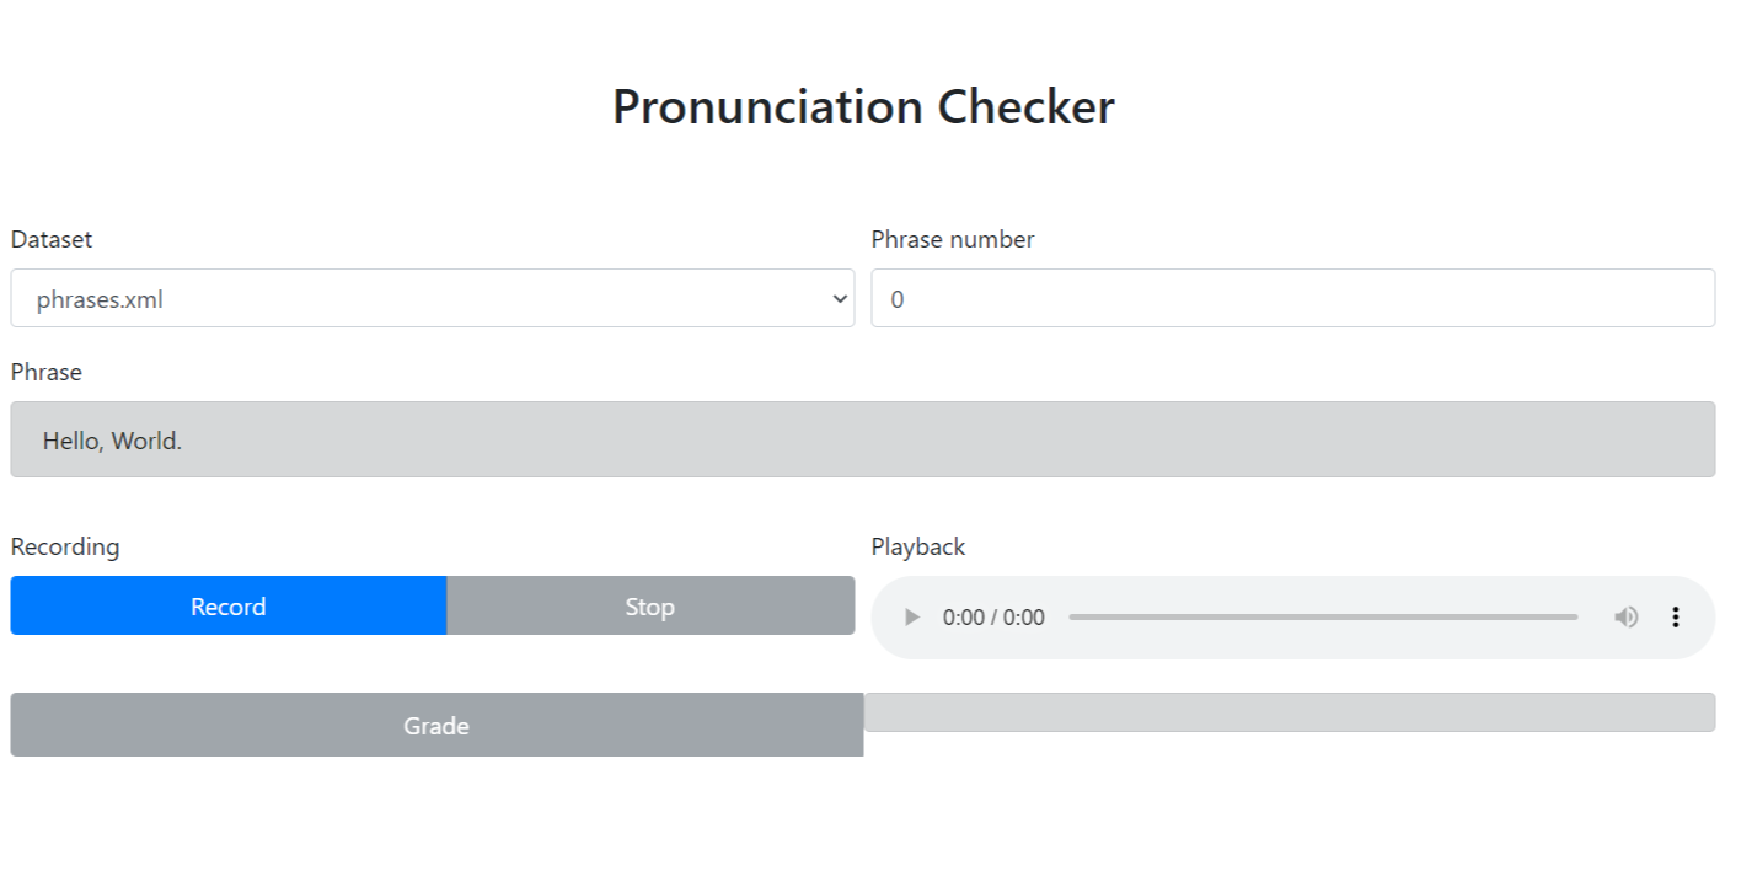
\includegraphics[scale=0.55]{images/homepage.pdf}
    \caption{Application's web page.}
\end{figure}

\end{document}
